\documentclass[conference]{IEEEtran}
\usepackage{cite}
\usepackage{amsmath,amssymb,amsfonts}
\usepackage{algorithmic}
\usepackage{graphicx}
\usepackage{textcomp}
\usepackage[dvipsnames]{xcolor}
\usepackage{caption}
\usepackage{matlab-prettifier}
\usepackage{siunitx}
\def\BibTeX{{\rm B\kern-.05em{\sc i\kern-.025em b}\kern-.08em
    T\kern-.1667em\lower.7ex\hbox{E}\kern-.125emX}}


\begin{document}

\title{CMP9135M | Computer Vision}

\author{\IEEEauthorblockN{1\textsuperscript{st} George Davies}
    \IEEEauthorblockA{
        \textit{School of Computer Science} \\
        \textit{University of Lincoln}\\
        Lincoln, United Kingdom \\
        27421138@students.lincoln.ac.uk
    }
}

\maketitle

\section*{Task 1 | Image Processing}
    %Download two files: ‘ball_frames.zip’ from Blackboard. Unzip the dataset file, you should obtain a set of 126 images. 
    %Among those images, there are 63 ball colour images and 63 corresponding ball mask images (ground-truth segmentation). 
    %Figure 1 shows an example of one ball image and its corresponding mask image. Please use conventional computer vision 
    %techniques (no deep/machine learning solution allowed in this task) to implement the following tasks. Please note that
    % you are expected to develop one model with same parameter settings for all the images.

    The aim of this task was to segment three different types of balls (a tennis ball, a football, and an american football) from a timeseries of
    images of them rolling across the frame. No deep learning solutions were allowed.

    \subsection*{Task 1.a | Automated ball objects segmentation}
        %Automated ball objects segmentation. For each image, automatically segment the balls from background.
        \subsubsection{Otsu thesholding}
        The first step was to binarise the image. By default, the matlab function imbinarize uses otsu to distinguish between foreground and 
        background. \\
        By ajusting the sensitivity, I found the value that removed the most of the background without removing the balls was 0.35.\\
        The imbinarize function only works on grayscale images so I tested parsing each colour channel separately and the red channel seemed to 
        perform the best. \\
        Examples of the output can be seen in Figure~\ref{fig:otsu}.

        \begin{figure}[htbp]
            \centering
            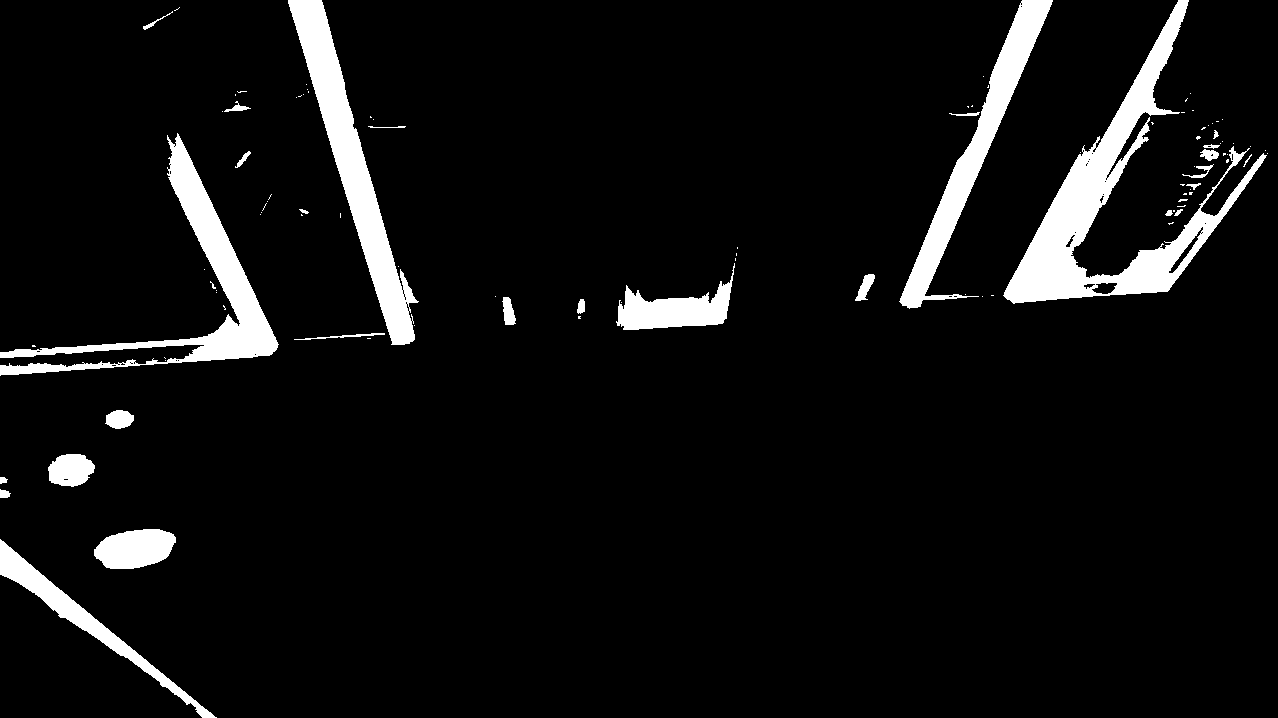
\includegraphics[width=0.49\columnwidth]{figures/otsu_mask.png}
            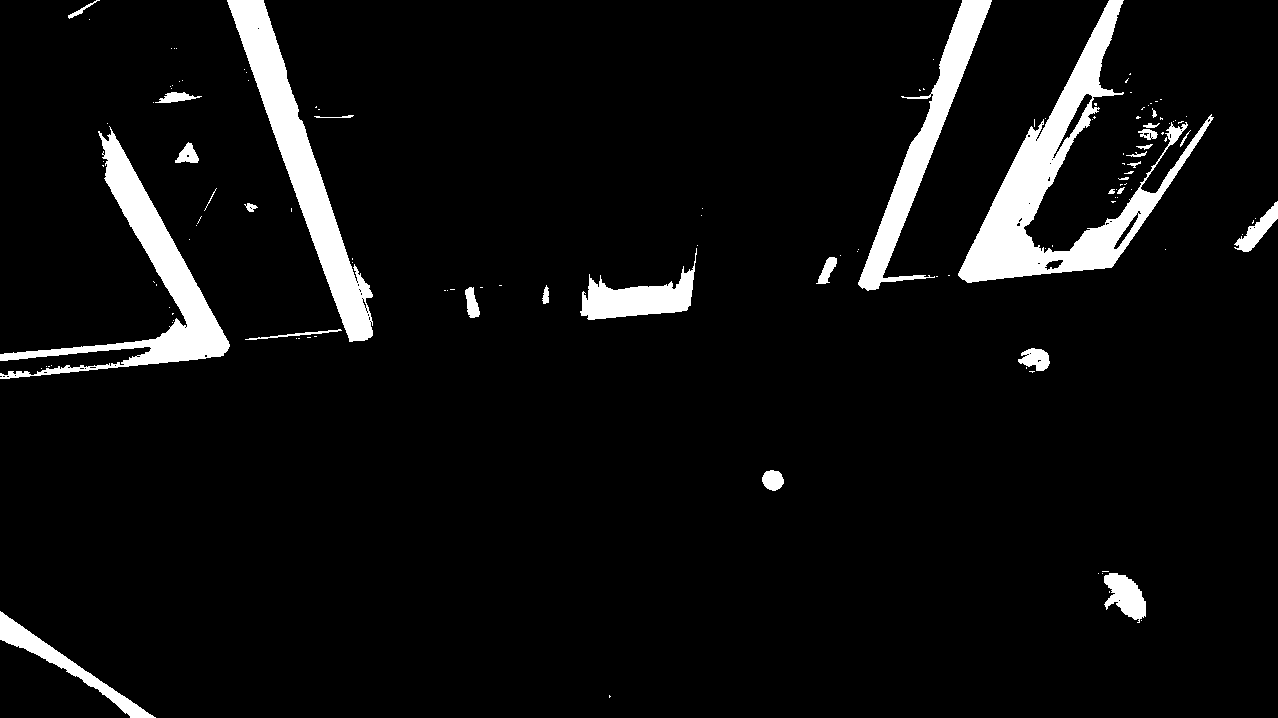
\includegraphics[width=0.49\columnwidth]{figures/otsu_mask2.png}
            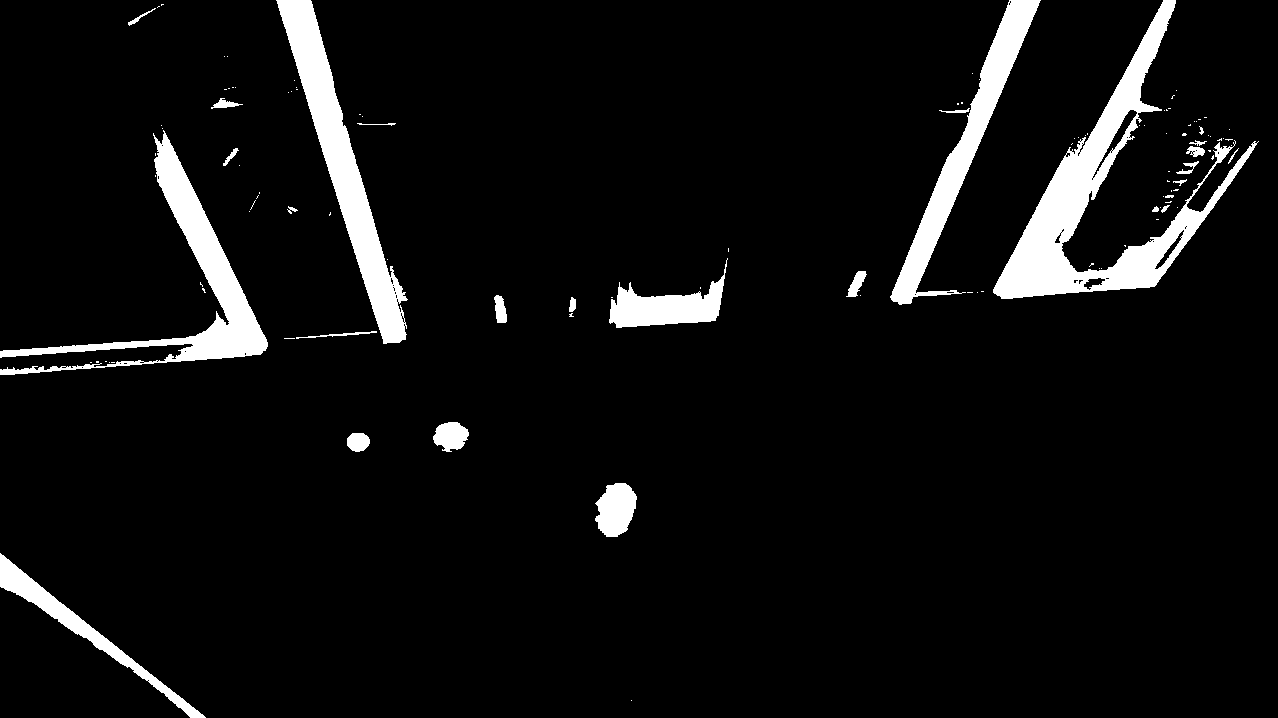
\includegraphics[width=0.49\columnwidth]{figures/otsu_mask3.png}
            \caption{Examples of the binary image output of the preliminarly segmentation using otsu~\label{fig:otsu}}
        \end{figure}

        \subsubsection{Converting to convex hulls}

        To removed the remaining background artifacts, I decided to convert all the connected components into convex hulls. \\
        As the ball are supposed to be convex in the first place, they shouldn't change much (apart from the american football in the last few 
        frames where the otsu segmentation was a bit aggressive). \\
        This had the effect of massivly increasing the area of the background artifacts, making them 
        easily distinguishable from the balls. \\
        Examples of the output can be seen in Figure~\ref{fig:convex}.

        \begin{figure}[htbp]
            \centering
            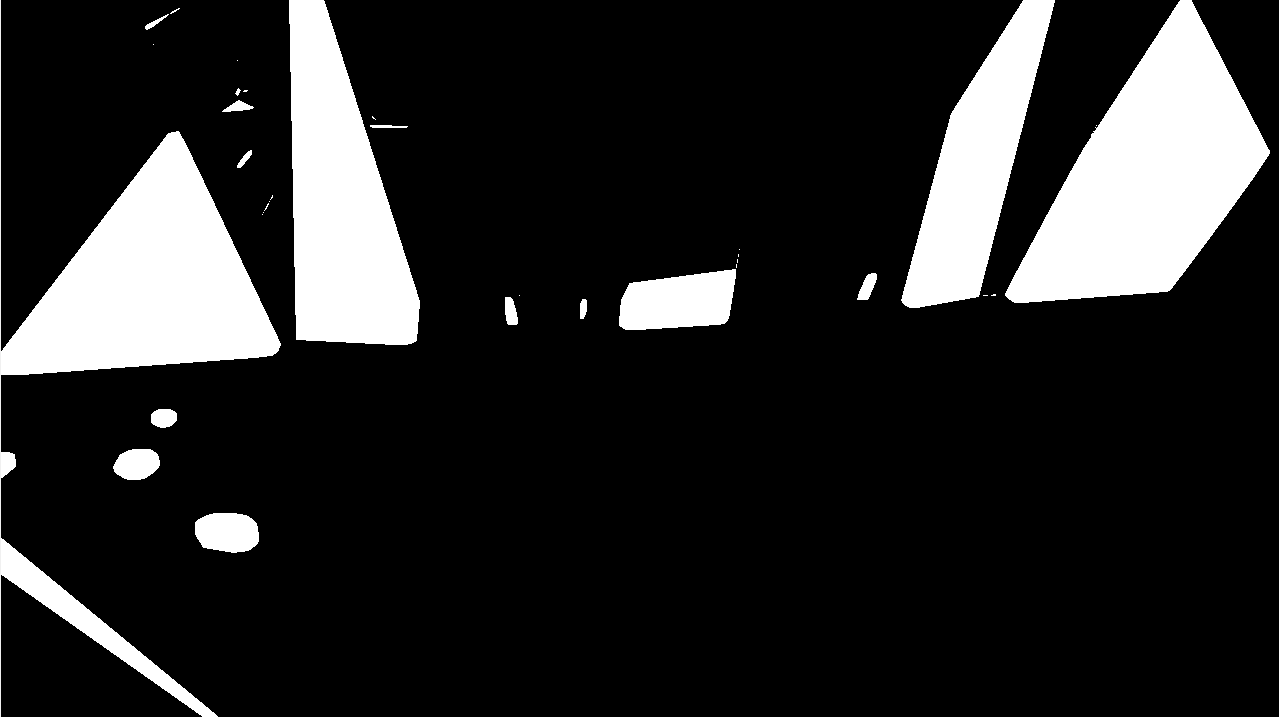
\includegraphics[width=0.49\columnwidth]{figures/convex3.png}
            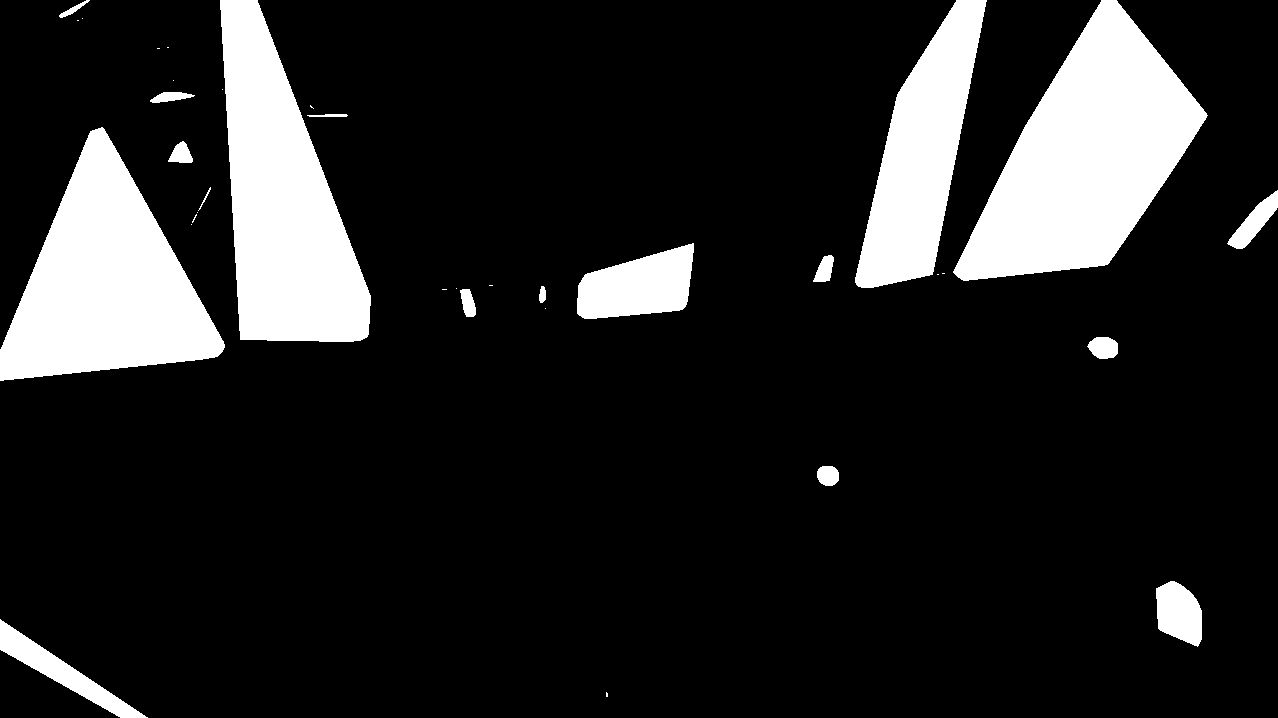
\includegraphics[width=0.49\columnwidth]{figures/convex2.png}
            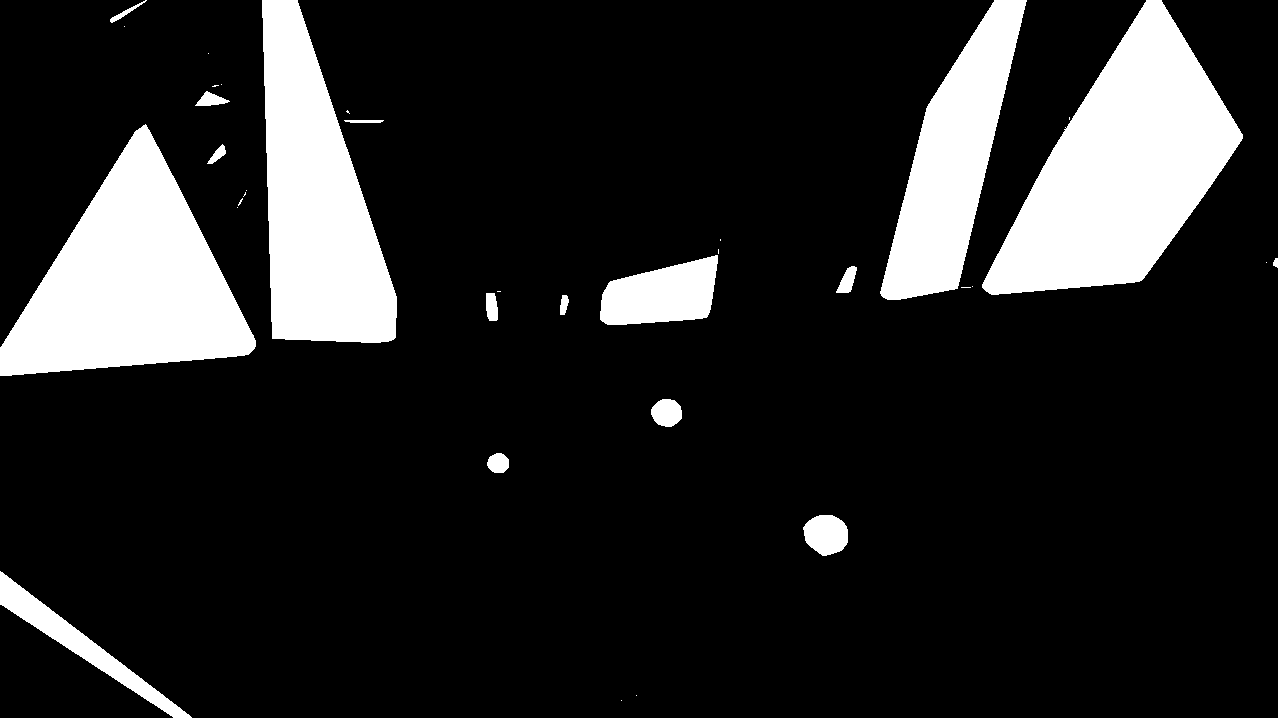
\includegraphics[width=0.49\columnwidth]{figures/convex.png}
            \caption{Examples of the binary image output after transforming each connected component into a convex hull~\label{fig:convex}}
        \end{figure}

        \subsubsection{Removing the remaining artifacts}

        Now, the background artifacts can be removed from the binarised images by removing every connected component that doesn't fit certain
        characteristics such as area and extent.
        After this, all that remains are the three balls.


        \begin{figure}[htbp]
            \centering
            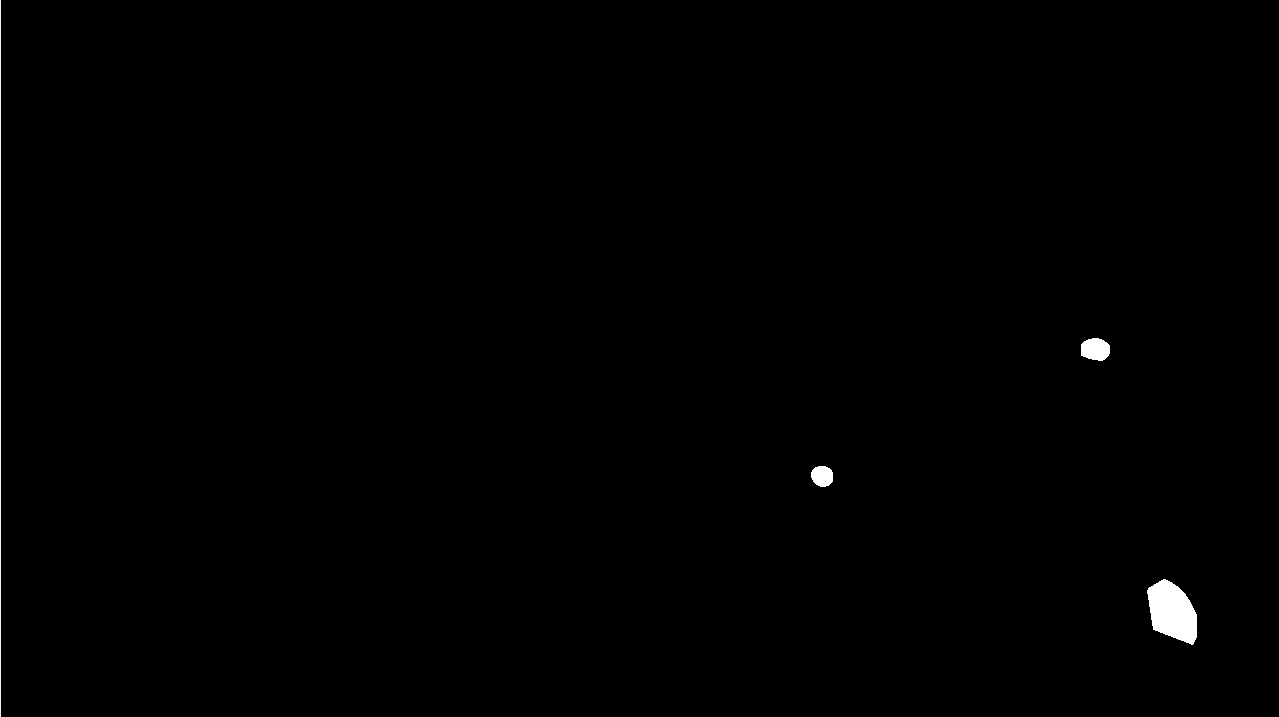
\includegraphics[width=0.49\columnwidth]{figures/final_mask.png}
            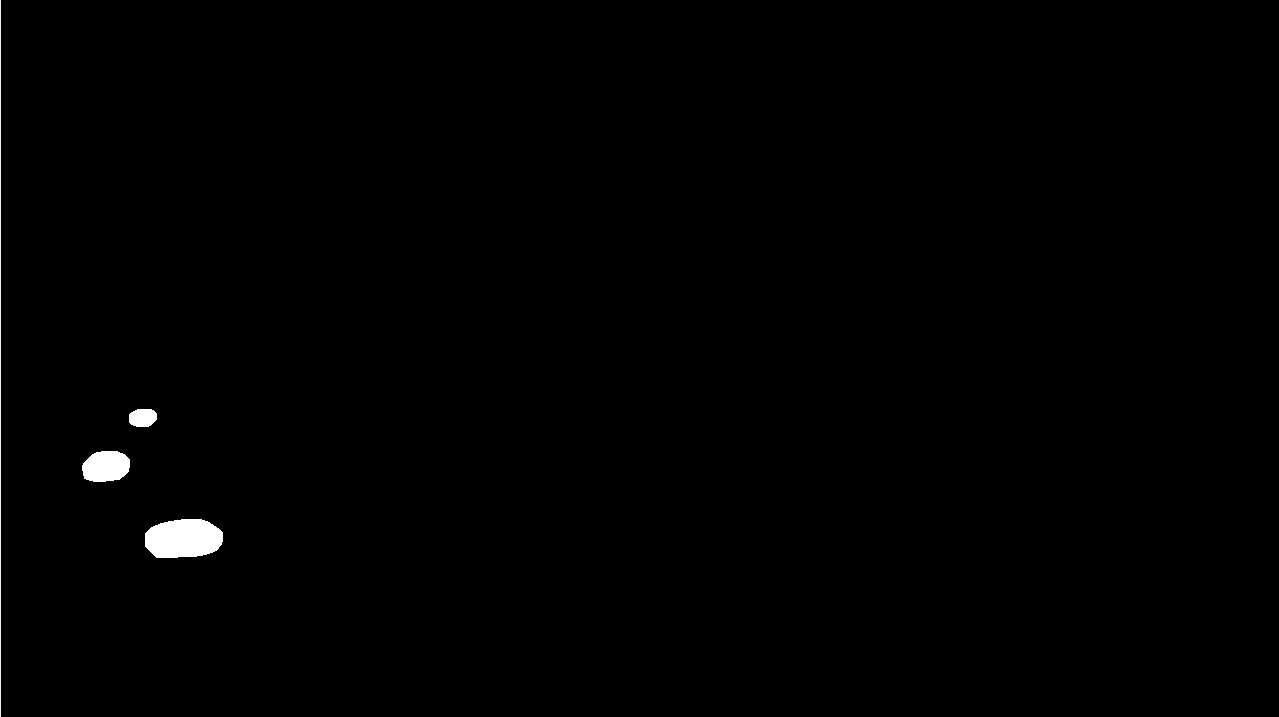
\includegraphics[width=0.49\columnwidth]{figures/final_mask2.png}
            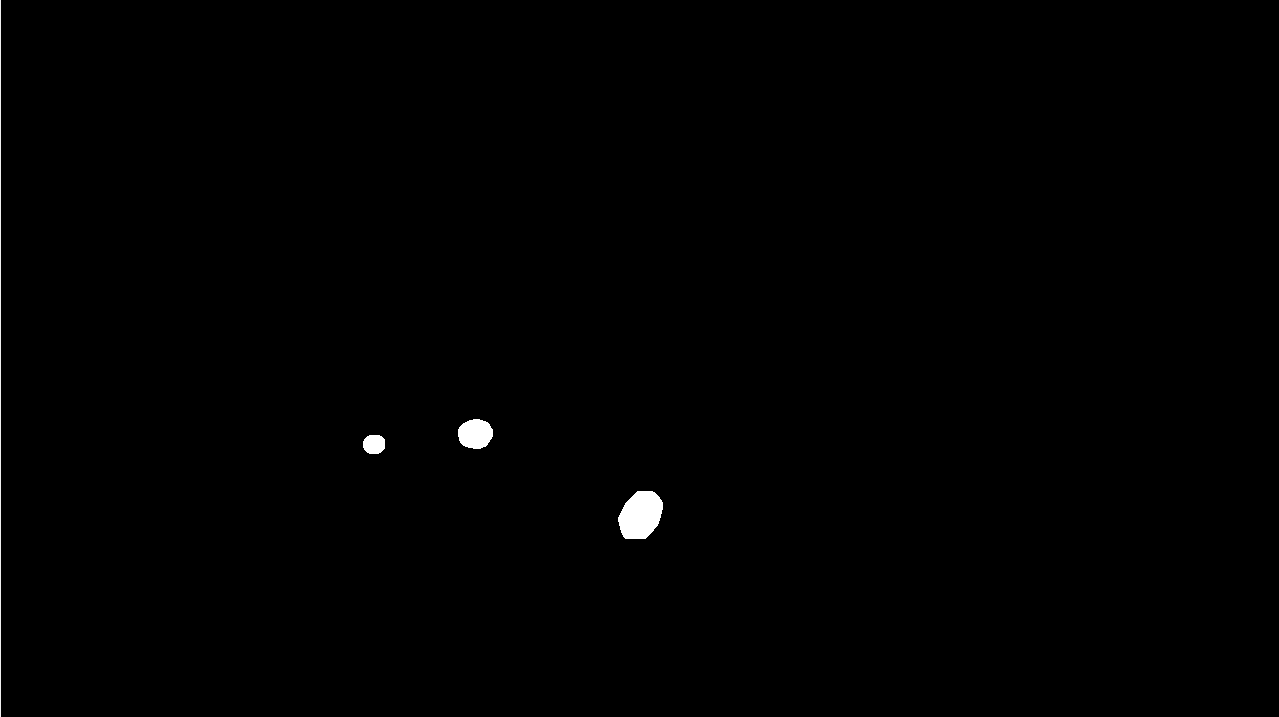
\includegraphics[width=0.49\columnwidth]{figures/final_mask3.png}
            \caption{Examples of the binary image output after transforming each connected component into a convex hull~\label{fig:final}}
        \end{figure}

        More examples of the best and worst segmentations can be found in the Appendix Figures~\ref{apx:best} and~\ref{apx:worst}


    \subsection*{Task 1.b | Segmentation evaluation}
        %Segmentation evaluation. For each ball image, calculate the Dice Similarity Score (DS) which is defined in Equation 1;
        %where M is the segmented ball region you obtained from Task 1, and S is the corresponding ground-truth binary ball 
        %mask. Please note that, in this case, for the provided ball mask images, you can convert the grayscale images into 
        %binary images (e.g. ball object and background), and use the converted binary images as ground-truth mask.

        %The calculated DS shall be between 0 and 1. For example, DS is 1 if your segmentation matches perfectly with the 
        %ground-truth mask, whist DS is 0 if there is no overlap between your segmentation and ground-truth mask.

        %Your report should include: 1) for all the 63 ball images, please provide a bar graph with x-axis representing the 
        %number of the image, and y-axis representing the corresponding DS. 2) calculate the mean and standard deviation of the
        %DS for all the 63 images, and 3) briefly describe and justify the implementation steps. Please note that you are 
        %required to show the best 5 and worst 5 segmented ball images (along with the corresponding ball GT mask images) in 
        %the Appendix.

        To evaluated the segmentation, the Dice Similarity score between the segmented images and the ground truth can be calculated.
        As each image is simply stored as a matrix of 1s and 0s, it is possible to do binary operations on the matrices.
        The DS score is calculated by multiplying the number of 1s in the intersection of the two matrices (logical \&) by 2 and dividing 
        that by the total number of 1s in both matrices. If there is a perfect overlap between the images, then the intersection will 
        incompass all the 1s and the DS score will be 1. If there is no overlap, then there is no intersection and the DS score will be 0.

        \begin{equation}
            \text{Dice}(M, S) = \frac{2|M \cap S|}{|M| + |S|}
        \end{equation}
        where:
        \begin{itemize}
            \item M and S are the to sets to compared
            \item $|$M$|$ and $|$S$|$ are sizes of the sets M and S
        \end{itemize}
            

        \begin{figure}[htbp]
            \centering
            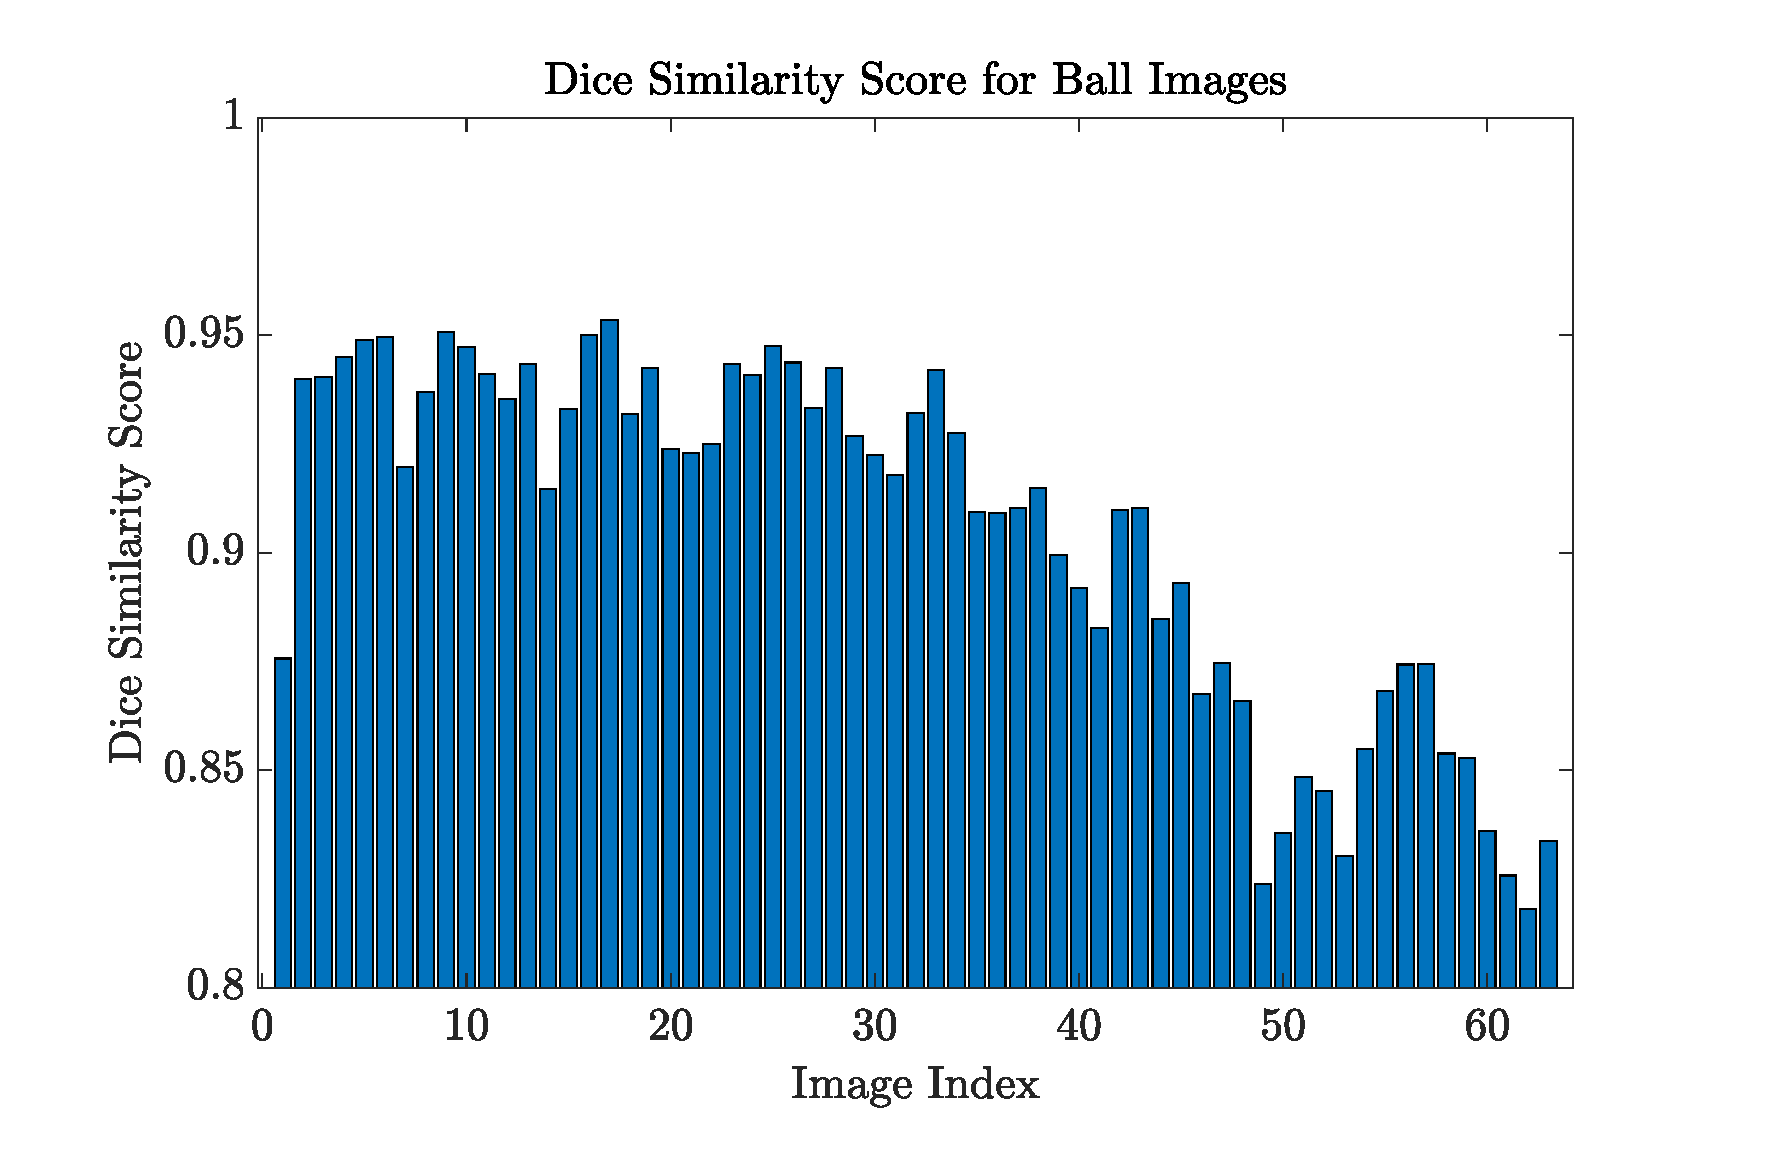
\includegraphics[width=\columnwidth]{figures/DS_bar_graph.pdf}
            \caption{Dice Similarity score for all 63 images.\ y-axis restricted between 0.8 and 1 for better visibility~\label{fig:DS_bar_graph}}
        \end{figure}

        As seen in Figure~\ref{fig:DS_bar_graph}, the segmentation performs well from images 2 to 34, then it starts to lower in quality.
        This is due to the otsu segmentation of the american football being too strong near the end.\\
        The average every image's DS score is \textbf{0.90464} and the standard deviation is \textbf{0.040538} 

\section*{Task 2 | Feature Calculation}
    %This part of the assignment will deal with feature extraction, more specifically you will be examining texture and 
    %shape features. Using the provided GT ball masks to obtain the corresponding ball patches from original RGB images, 
    %carrying out the following tasks.

    \subsection*{Task 2.a | Shape features}
        %For each of the ball patches, calculate four different shape features discussed in the lectures (solidity, 
        %non-compactness, circularity, eccentricity). Plot the distribution of all the four features, per ball type.

        For this task, the following shape features were calculated:
        \begin{enumerate}
            \item Solidity: The proportion of the pixels in the convex hull that are also in the object.
            \[\text{Solidity} = \frac{\text{Area of the object}}{\text{Area of its convex hull}}\]
            \item Non-compactness: Compactness is the proportion of the region's pixels to all of the bounding box's pixels. So non-compactness is the inverse of this.
            \[\text{Non-compactness} = 1 - \frac{\text{Area of the object}}{\text{Area of bounding box}}\]
            \item Circularity: The roundness of the object.
            \[\text{Circularity} = \frac{4\pi * \text{Area of the object}}{{(\text{Perimeter of the object})}^2} * \left(1 - \frac{0.5}{{\text{r}}}\right)\]
            Where r = $\frac{\text{Perimeter of the object}}{2\pi} + 0.5$
            \item Eccentricity: The eccentricity is the proportion of the distance between the foci of the ellipse and the length of its major axis. An eccentricity of 0 means its a perfect circle. An eccentricity of 1 means its a line.
            \[\text{Eccentricity} = \frac{\text{Distance between foci of ellipse}}{\text{Length of major axis of ellipse}}\]
        \end{enumerate}


        \begin{figure}[htbp]
            \captionsetup{singlelinecheck=off}
            \centering
            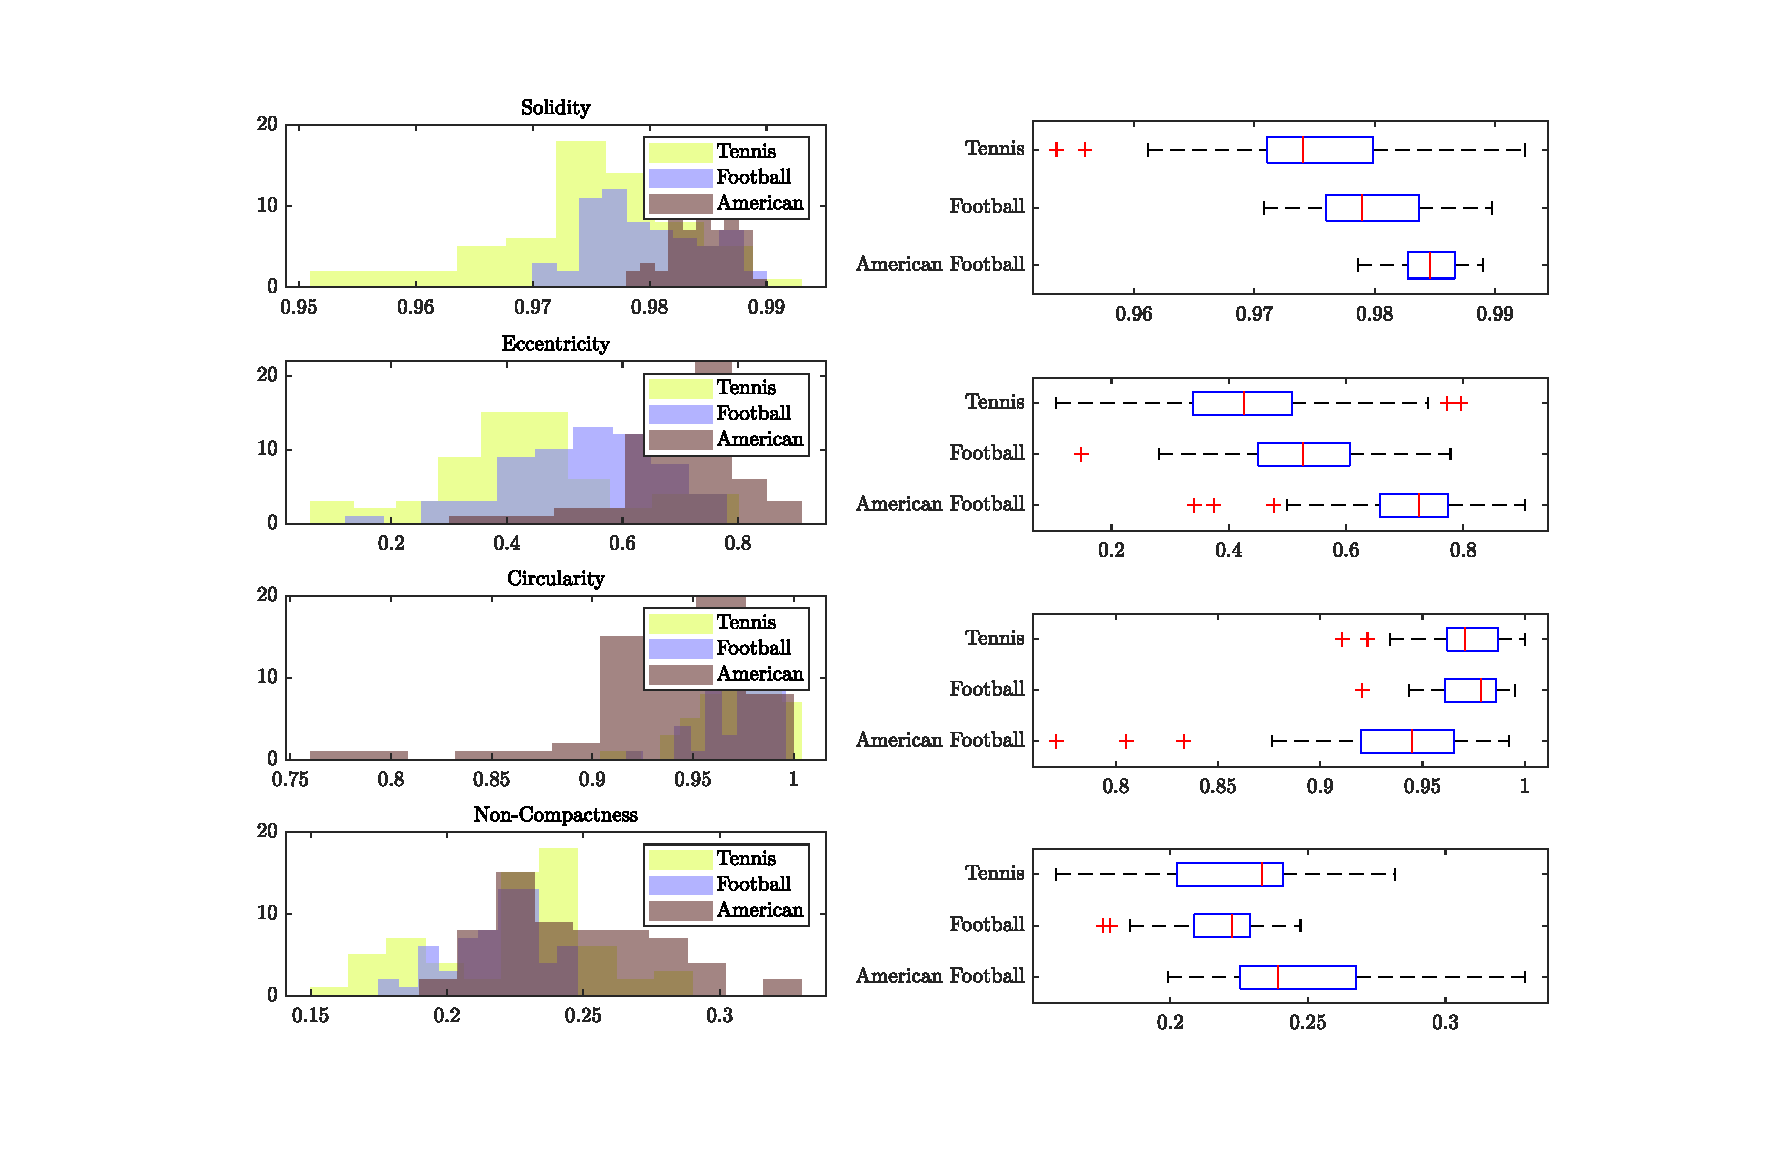
\includegraphics[width=\columnwidth]{figures/shape_feats.pdf}
            \caption[]{Histograms and boxplots showing the Solidity, Non-Compactness, Circularity, and Eccentricity of the three ball types.\\
                Legend: 
                \begin{itemize}
                    \item \textcolor{Dandelion}{yellow}: tennis
                    \item \textcolor{CadetBlue}{blue}: football
                    \item \textcolor{Tan}{brown}: american football
                \end{itemize}~\label{fig:shape_feats}
            }
        \end{figure}

        Figure~\ref{fig:shape_feats} displays histograms and boxplots representing the distribution of four different shape features (solidity, non-compactness, circularity, and eccentricity) for each ball type (tennis, football, and American football).\\
        Going through each shape feature one by one. 

        There is a lot of overlap between the three ball types for solidity. 
        The tennis ball has the lowest median solidity, followed by the football, and then the American football. 
        The tennis ball has the highest range of solidity values, followed by the football, and then the american football. 

        For Eccentricity, the order of the median values is the same as for solidity but there is less overlap between the three ball types.
        This measure seems better at distinguishing the american football from the other two ball types as the american football is not a sphere like the other two balls.

        Circularity like eccentricity is better at distinguishing the american football from the other two ball types, with the tennis ball and football having a similar Q1 and Q3 values.
        This is also due to the american football not being a sphere like the other two balls.

        Finally, non-compactness is the worst at distinguishing between the three ball types as there is a lot of overlap between the three ball types.
        The mean of the non-compactness values for each ball lie within 0.025 of each other.

    \subsection*{Task 2.b | Texture features}
        %Calculate the normalised grey-level co-occurrence matrix in four orientations (0°, 45°, 90°, 135°) for the patches 
        %from the three balls, separately for each of the colour channels (red, green, blue). For each orientation, calculate 
        %the first three features proposed by Haralick et al. (Angular Second Moment, Contrast, Correlation), and produce 
        %per-patch features by calculating the feature average and range across the 4 orientations. Select one feature from 
        %each of the colour channels and plot the distribution per ball type.
        The goal of this task was to calculate the normalised grey-level co-occurrence matrix (glcm) in 4 orientations for each ball patch 
        and for each colour channel.

        The texture features that were extracted were:
        \begin{itemize}
            \item Angular Second Moment (ASM): also know as energy is the sum of squared elements in the glcm.\@
                \begin{equation}
                    \text{ASM} = \sum_{i,j} {p(i,j)}^2
                \end{equation}
            \item Contrast: is the a measure of the intensity contrast between a pixel and its neighbor over the whole image.
                \begin{equation}
                    \text{Contrast} = \sum_{i,j} |i-j|^2 p(i,j)
                \end{equation}
            \item Correlation: is the measure of how correlated a pixel is to its neighbor over the whole image.
                \begin{equation}
                    \text{Correlation} = \sum_{i,j} \frac{(i-\mu_i)(j-\mu_j)p(i,j)}{\sigma_i \sigma_j}
                \end{equation}
        \end{itemize}

        For each of these texture features, the average and range was calculated over the four orientations 
        (\ang{0}, \ang{45}, \ang{90}, \ang{135}).\\
        The averages can be seen in Figure~\ref{fig:tex_feats_avgs} and the ranges can be seen in Figure~\ref{fig:tex_feats_ranges}

        \begin{figure}[htbp]
            \centering
            \captionsetup{singlelinecheck=off}
            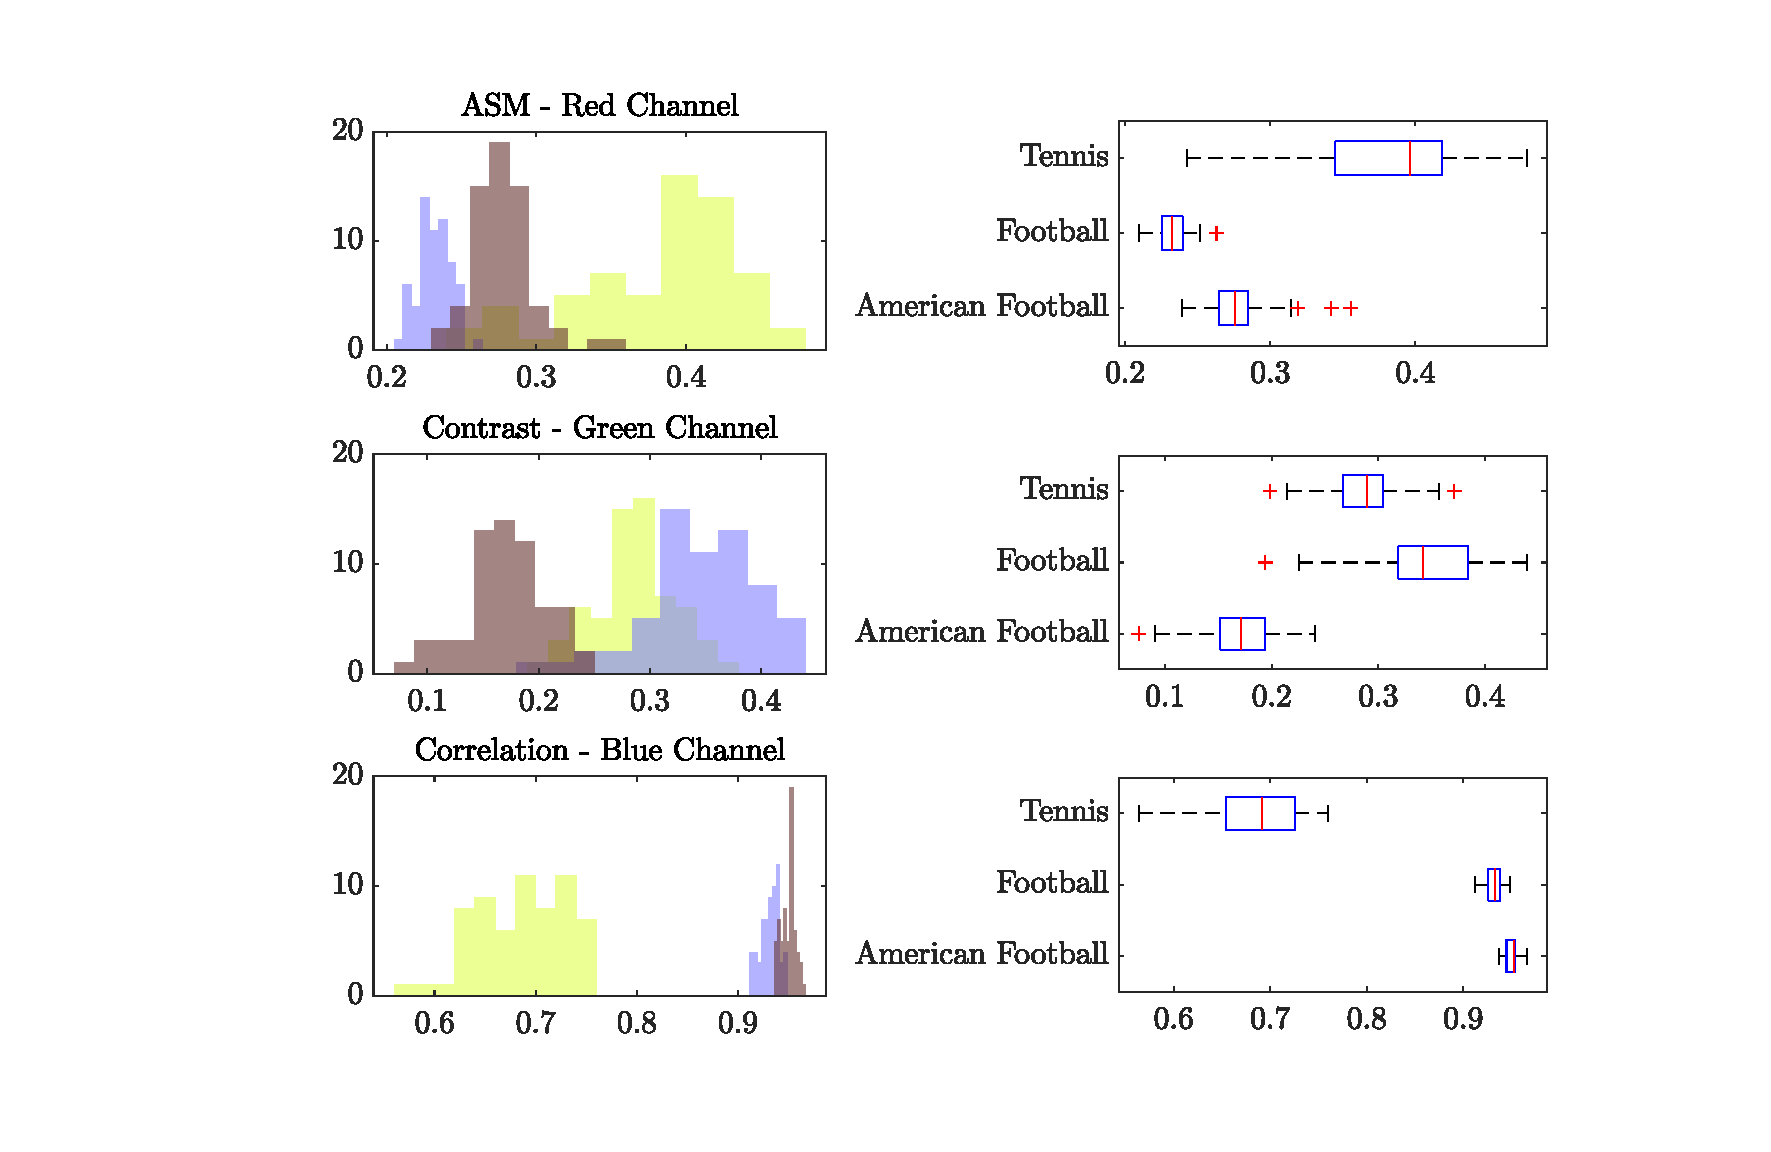
\includegraphics[width=\columnwidth]{figures/averages.pdf}
            \caption[]{Histograms and boxplots showing the average Angular Second Moment, Contrast, and Correlation associated with one colour channel for each ball type.
                Angular Second Moment on the red channel,
                Contrast on the green channel,
                Correlation on the blue channel. Same Legend as Figure~\ref{fig:shape_feats}.~\label{fig:tex_feats_avgs}
            }
        \end{figure}

        For ASM in the red channel, there is no overlap between the ball types from their Q1 to Q3. Meaning this is a very good metric for 
        discriminating between the ball types.\\
        Same goes for Contrast in the green channel though there is more overlap between the tennis ball and football. The american football
        is very distinguished from the other ball types.\\
        Finally for the Correlation in the blue channel, the tennis ball is completely seperated from the other two ball types with minor
        overlap between the football and american football.

        \begin{figure}[htbp]
            \centering
            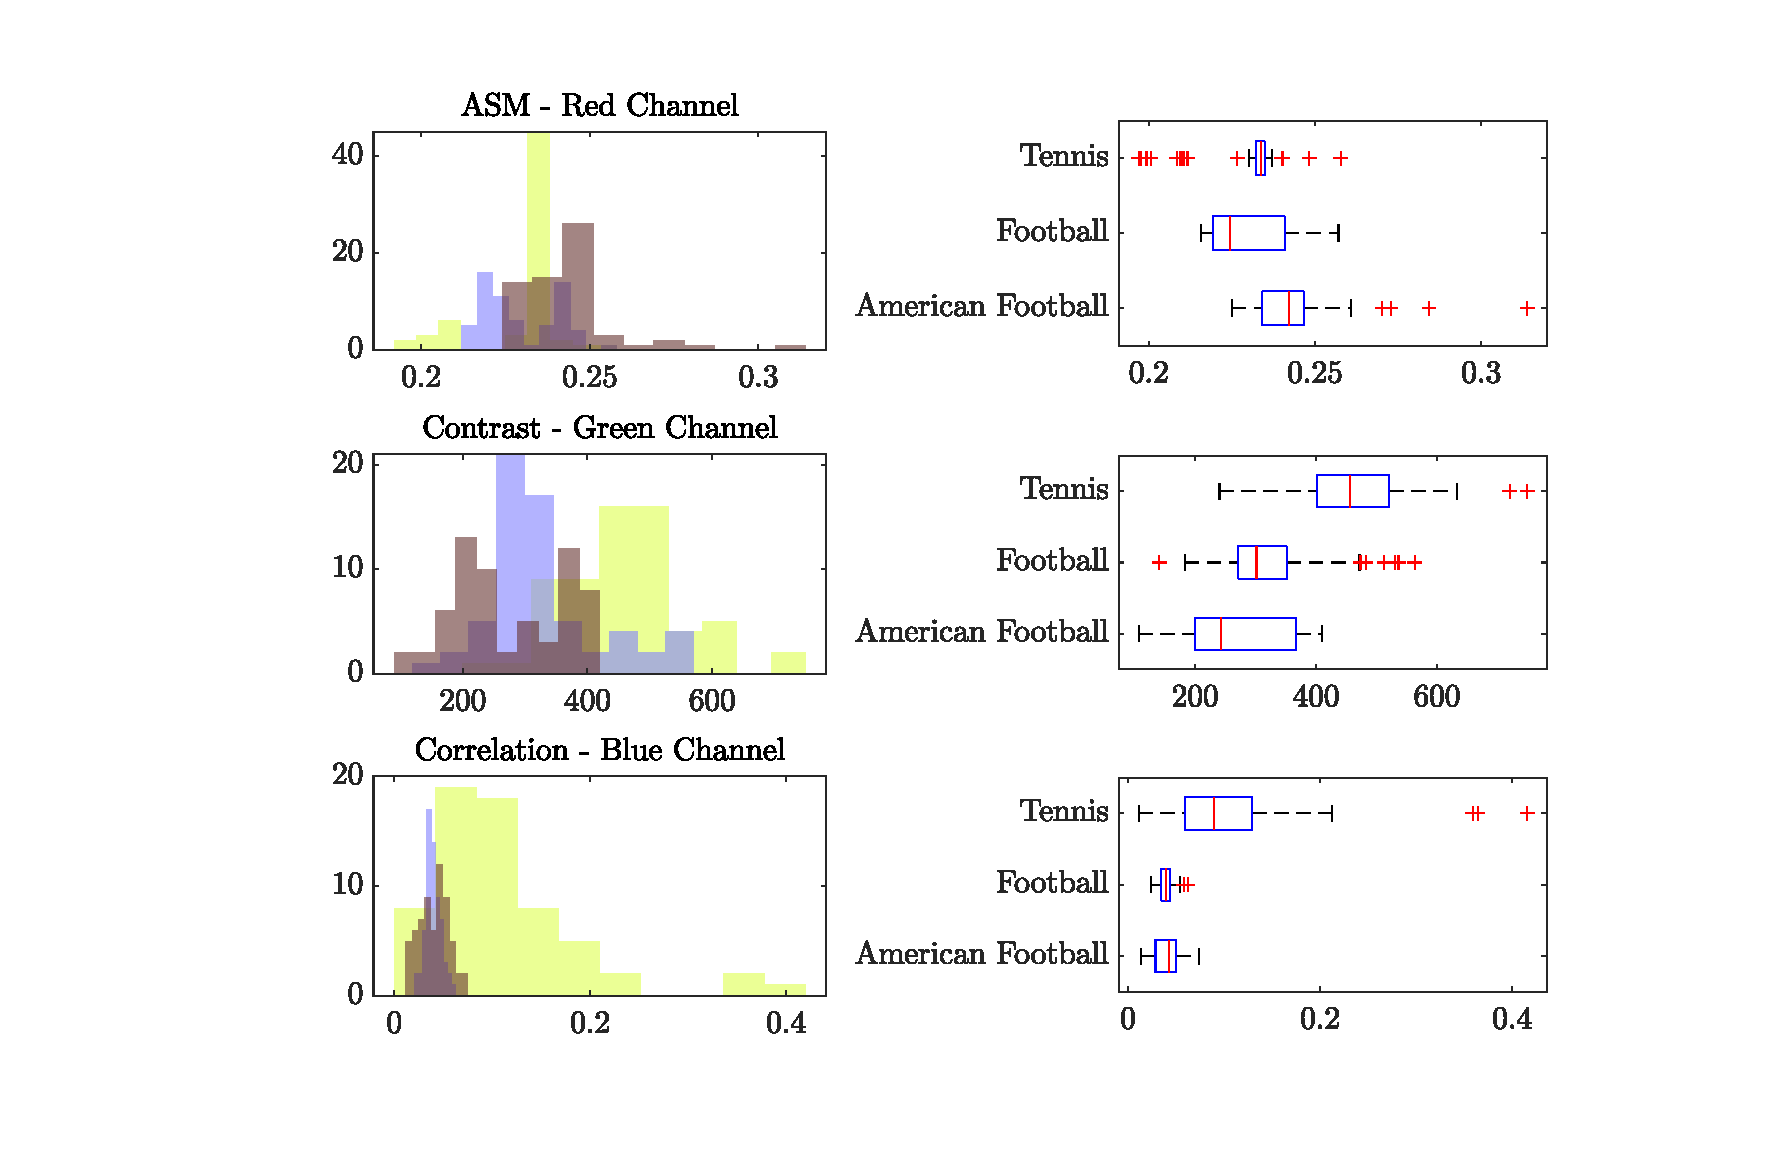
\includegraphics[width=\columnwidth]{figures/ranges.pdf}
            \caption[]{Histograms and boxplots showing the ranges of Angular Second Moment, Contrast, and Correlation associated with one colour channel for each ball type.
                Angular Second Moment on the red channel,
                Contrast on the green channel,
                Correlation on the blue channel. Same Legend as Figure~\ref{fig:shape_feats}.~\label{fig:tex_feats_ranges}
            }
        \end{figure}

        With the ranges instead of the averages, the ASM seperates the three balls relativly well with the tennis ball frequently having a value
        of zero and the two others with a small amount of overlap.\\
        The Contrast is very bad at distinguishing the tennis ball from the american football, with the regular football having slightly higher 
        contrast.\\
        The Correction is incapable of distinguishing the tennis ball but is alright at seperating the football from the american football.


    \subsection*{Task 2.c | Discriminative information}
        %Based on your visualisations in part a) and b), discuss which features appear to be best at differentiating between 
        %different ball types. For each ball type, are shape or texture features more informative? Which ball type is the 
        %easiest/hardest to distinguish, based on the calculated features? Which other features or types of features would you 
        %suggest for the task of differentiating between the different ball types and why?
        %Analyse and discuss your findings in the report.
        Overall the texture features are much better at providing discriminative information than the shape features. This makes sense
        for this situation as the three balls have similar shapes but their colours and patterns are more unique. If all three balls 
        were made out of the same material, the texture features would be much less effective.



\section*{Task 3 | Object Tracking}
    %Download from Blackboard the data files 'x.csv' and 'y.csv', which contain the real coordinates [x,y] of a moving 
    %ball, and the files 'na.csv' and 'nb.csv', which contain their noisy version provided by some segmentation and 
    %recognition for the football (e.g. frame-to-frame image segmentation of the target). Implement a Kalman filter from 
    %scratch (not using any method/class from pre-built libraries) that accepts as input the noisy coordinates [na,nb] and 
    %produces as output the estimated coordinates [x*,y*]. For this, you should use a Constant Velocity motion model F with 
    %constant time intervals Δt = 0.5 and a Cartesian observation model H.

    The final task was to implement a kalman filter from scratch without using any methods from inbuilt libraries. Four trajectories were given,
    x.csv and y.csv contained the real coordinates and na.csv and nb.csv contained the noisy coordinates from which estimated coordinates could 
    be calculated.
    
    For this task, certain variables were set:
    F is should be a Constant Velocity motion model.\ i.e.
    \begin{equation}
        \text{F} = \begin{bmatrix}
            1 & \Delta t & 0 & 0        \\
            0 & 1        & 0 & 0        \\
            0 & 0        & 1 & \Delta t \\
            0 & 0        & 0 & 1        \\
        \end{bmatrix}
    \end{equation}
    where $\Delta t$ is the time interval set to 0.5.\\
    H is a Cartisian observation model.\ i.e.
    \begin{equation}
        \text{H} = \begin{bmatrix}
            1&0&0&0\\
            0&0&1&0
        \end{bmatrix}
    \end{equation}
    The covariance matices Q and R are
    \begin{equation}
        \text{Q} = \begin{bmatrix}
            0.16 & 0 & 0 & 0 \\
            0 & 0.36 & 0 & 0 \\
            0 & 0 & 0.16 & 0 \\ 
            0 & 0 & 0 & 0.36 \\ 
        \end{bmatrix}
        \text{R} = \begin{bmatrix}
            0.25 & 0 \\ 
            0 & 0.25 \\ 
        \end{bmatrix}
    \end{equation}



    \subsection*{Task 3.a | Kalman filter tracking}
        %You should plot the estimated trajectory of coordinates [x*,y*], together with the real [x,y] and the noisy ones [a,b] 
        %for comparison. Discuss how you arrive to the solution.

        The kalman tracking algoritm iterates over every sample. For each sample, it predicts a state vector and a covariance using the constant 
        velocity motion model and the motion noise, with which it then estimates the state and covariance with the Cartesian observation model,
        observation noise, and the sample.\\
        Using the first sample and the initial state, Figure~\ref{fig:kalman} is the result
        \begin{figure}[htbp]
            \centering
            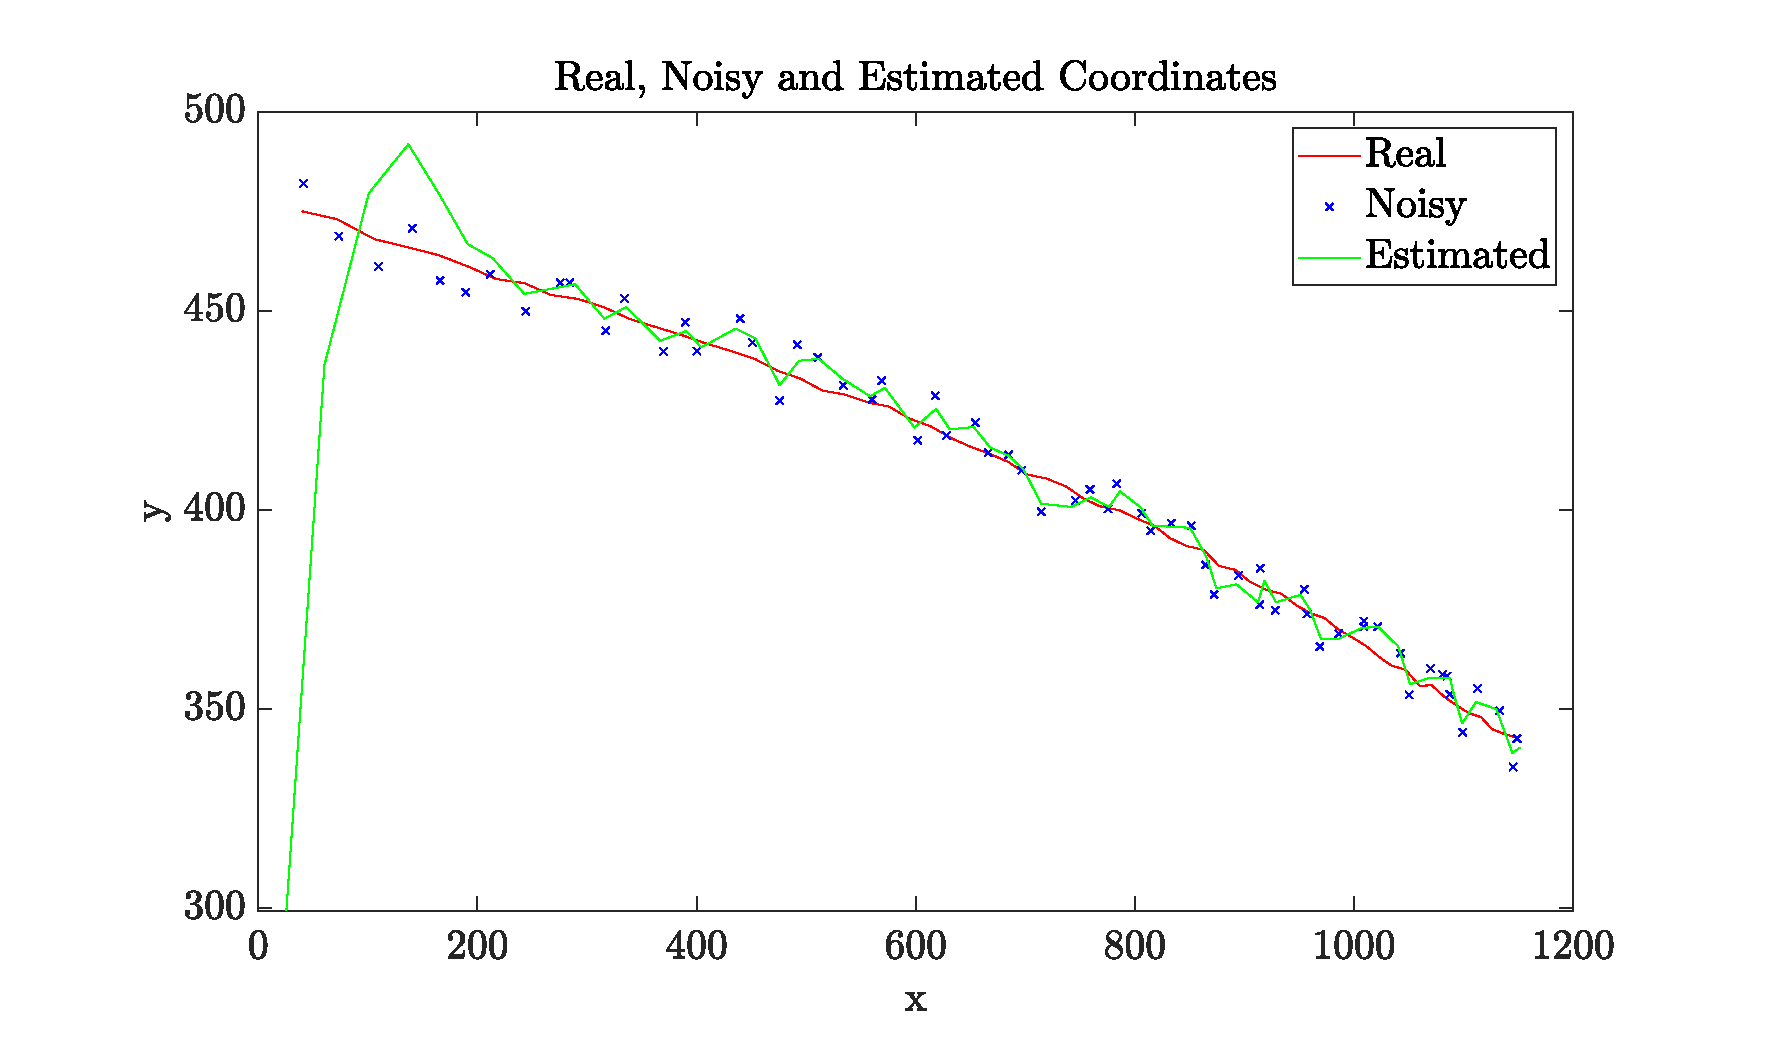
\includegraphics[width=\columnwidth]{figures/kalman.pdf}
            \caption{plot of the estimated trajectory of coordinates $[x\_, y\_]$, together with the real $[x,y]$ and the noisy $[na, nb]$ for comparison\label{fig:kalman}}
        \end{figure}

        \subsection*{Task 3.b | Evaluation}
        %You should also assess the quality of the tracking by calculating the mean and standard deviation of the Root Mean 
        %Squared error (include the mathematical formulas you used for the error calculation in your report). Compare both 
        %noisy and estimated coordinates to the ground truth. Adjust the parameters associated with the Kalman filter, justify
        % any choices of parameter(s) associated with Kalman Filter that can give you better estimation of the coordinates that
        % are closer to the ground truth. Discuss and justify your findings in the report.

        The equation for Root Mean Squared Error (RMSE) is:
        \begin{equation}
            \text{RMSE} = \sqrt{\frac{1}{n}\sum_{i=1}^{n}{({(x_i - \hat{x}_i)}^2 + {(y_i - \hat{y}_i)}^2)}}
        \end{equation}
        where:
        \begin{itemize}
            \item $n$ is the total number of observations
            \item $x_i \text{ and } y_i$ are the $i^{th}$ actual coordinates
            \item $\hat{x}_i \text{ and } \hat{y}_i$ is the $i^{th}$ predicted coordinates
        \end{itemize}
        This equation in matlab looks like this:
        \scriptsize
        % \lstset{basicstyle=\scriptsize}
        \begin{lstlisting}[style=Matlab-editor, basicstyle=\scriptsize]
    % Root Mean Squared Error (RMSE) calculation
    rmse_n = sqrt(mean((x - na).^2 + (y - nb).^2));
    rmse = sqrt(mean((x - x_).^2 + (y - y_).^2));
        \end{lstlisting}
        \normalsize
        $rsme\_n$ is the RMSE of the noisy coordinates relative to the ground truth.\\
        $rsme$ is the RMSE of the estimated coordinates realtive to the ground truth.


        \begin{equation}
            \sigma = \sqrt{\frac{1}{n}\sum_{i=1}^{n}{(x_i - \mu)}^2}
        \end{equation}    
        where:
        \begin{itemize}
            \item $\sigma$ is the standard deviation
            \item $n$ is the total number of observations
            \item $x_i$ is the $i^{th}$ value
            \item $\mu$ is the mean of the values
        \end{itemize}        
        This equation in matlab looks like this:
        \begin{lstlisting}[style=Matlab-editor, basicstyle=\scriptsize]
    % Standard deviation calculation of the RMSE
    std_n = std(sqrt((x - na).^2 + (y - nb).^2));
    std = std(sqrt((x - x_).^2 + (y - y_).^2));
        \end{lstlisting}
        \normalsize
        As the RMSE is a single number, there is no standard deviation. Therefore, I took the standard deviation of the root squared errors.

        The results of these calualations are:
        \begin{itemize}
            \item RMSE for the noisy coordinates \~= \textbf{7.416}
            \item RMSE for the estimated coordinates \~= \textbf{5.877}
            \item STD for the noisy coordinates \~= \textbf{2.573}
            \item STD for the estimated coordinates \~= \textbf{2.181}
        \end{itemize}
        All these values are relative to the real coordinates and rounded to the $3^{rd}$ decimal.
        These results show that the kalman filter successfully removed some of the noise as it is closer to the real coordinates.\\ 
        Better results may be found by testing different noise matrices and time intervals.
        

\appendix

    \begin{figure}[htbp]
        \centering
        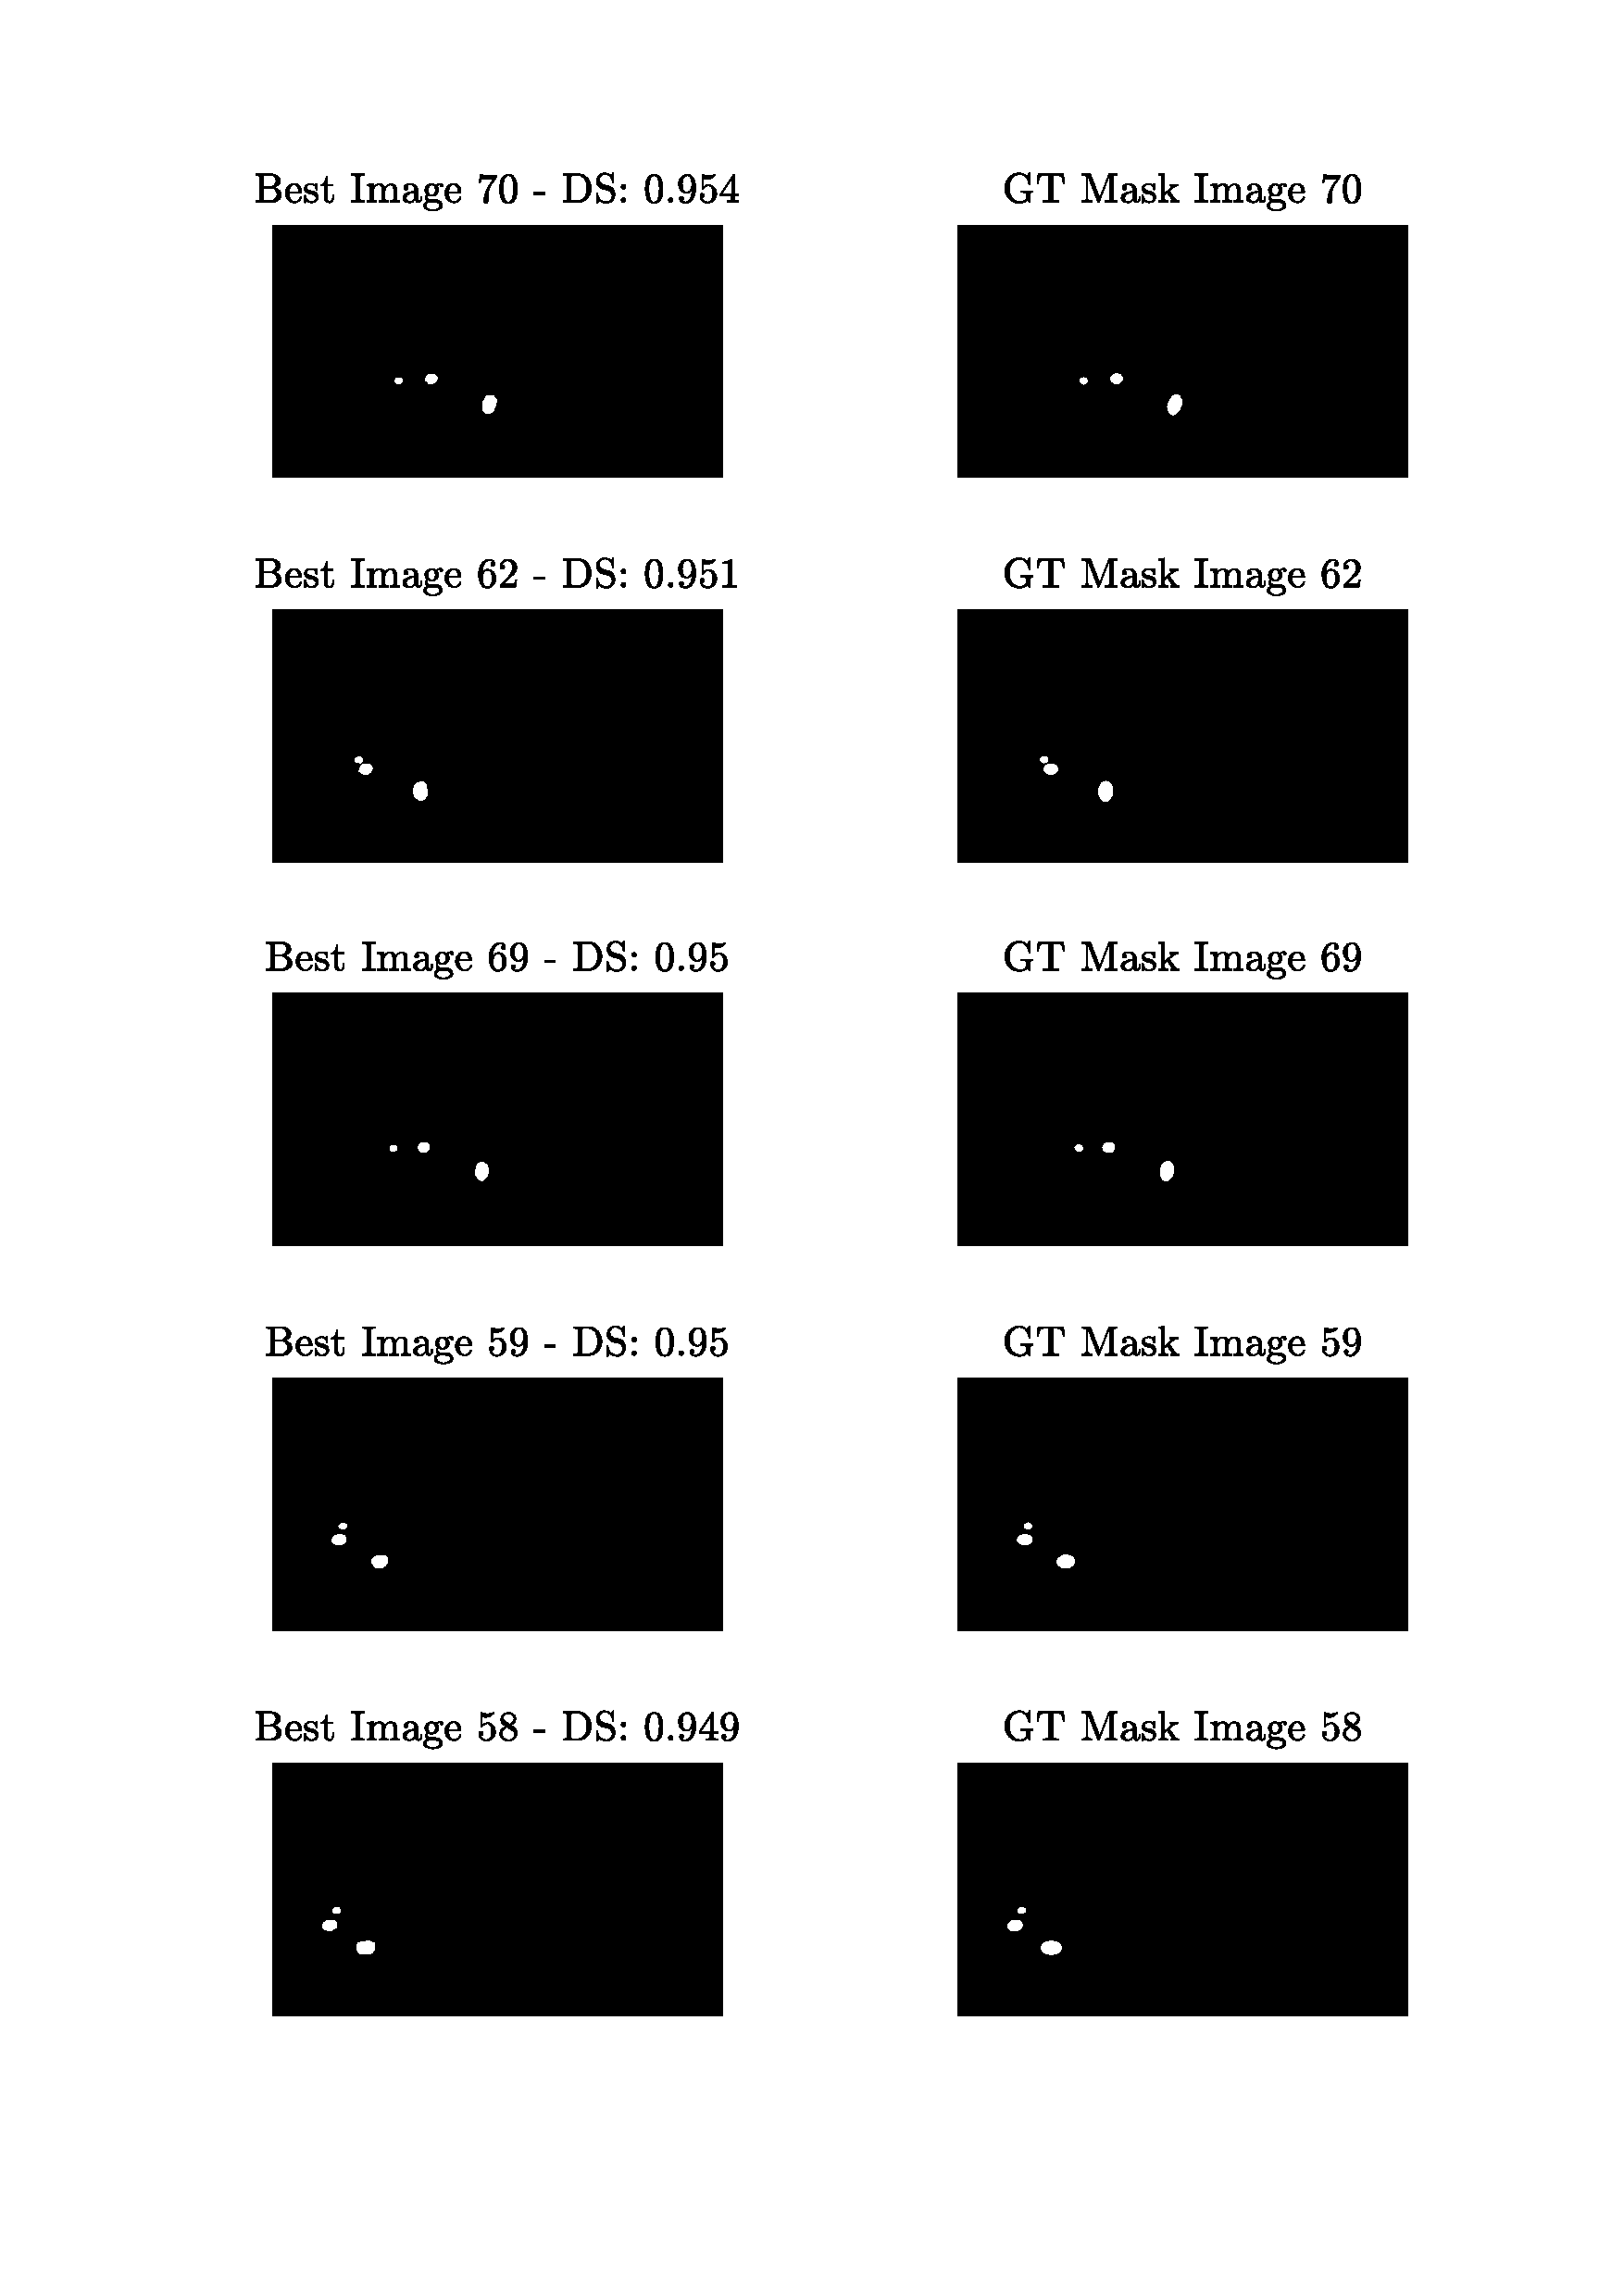
\includegraphics[width=\columnwidth]{figures/best.pdf}
        \caption{Best 5 segmented ball images compared to the ground truth\label{apx:best}}
    \end{figure}
    \begin{figure}[htbp]
        \centering
        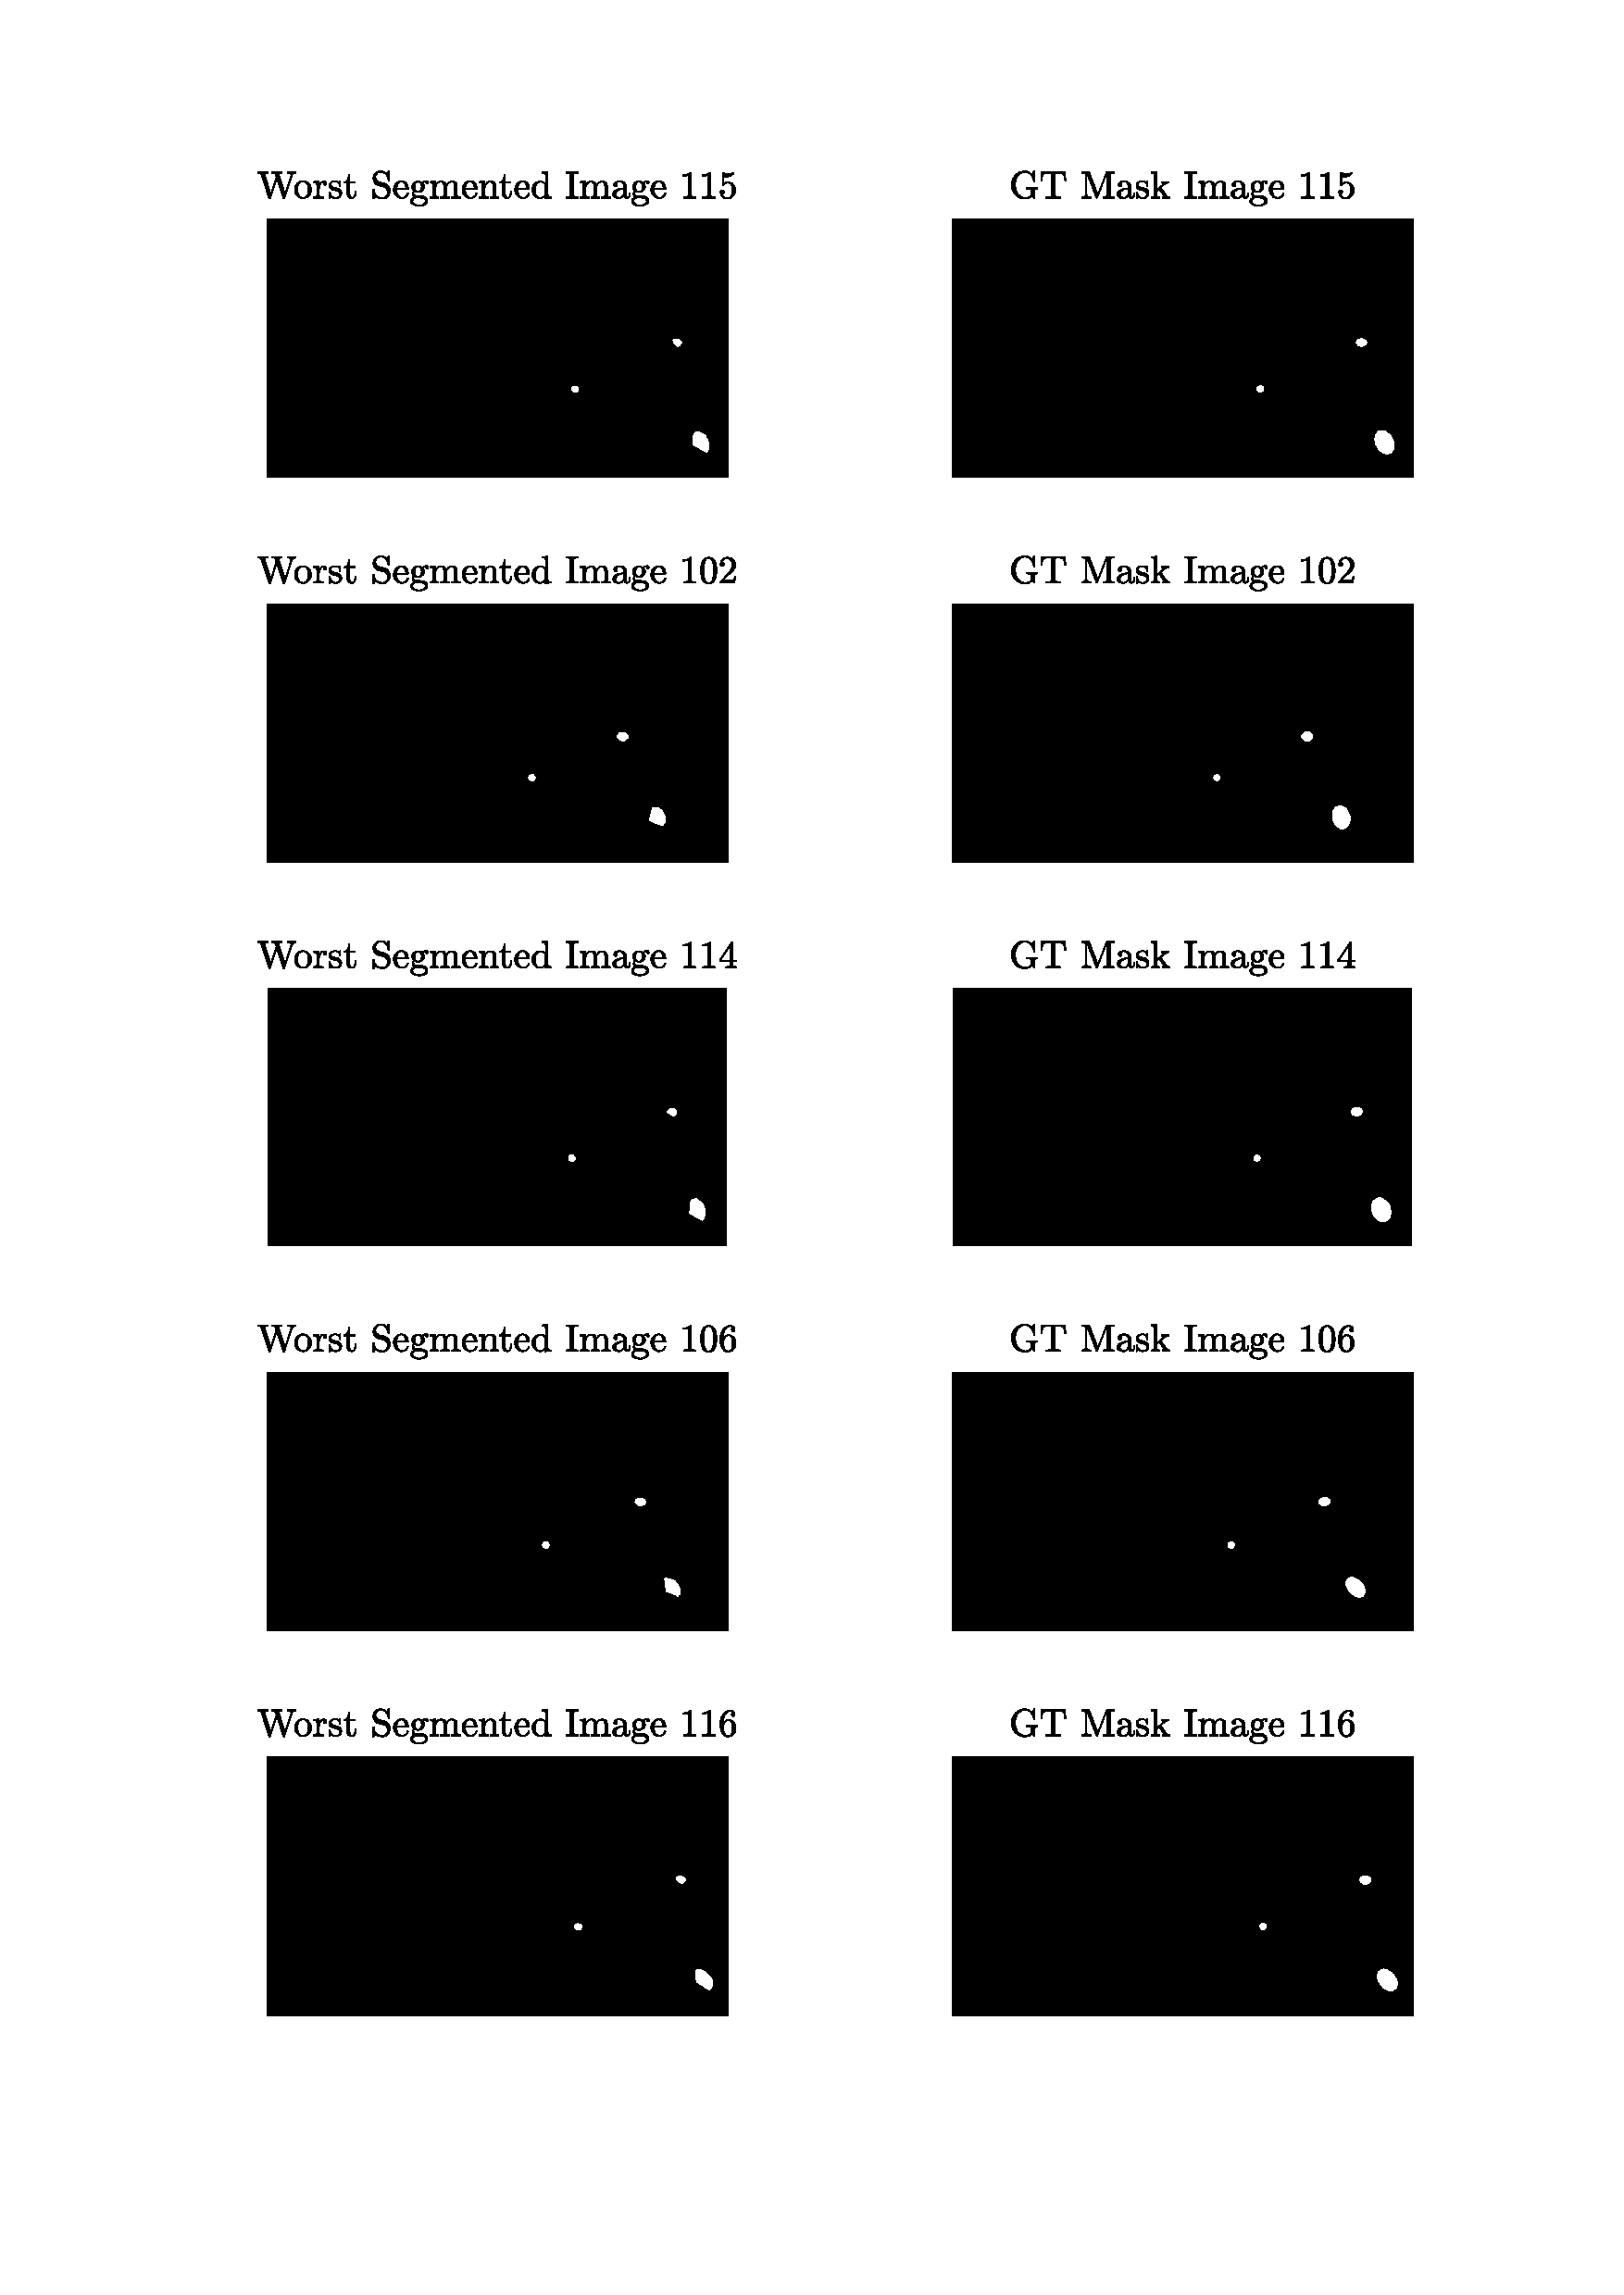
\includegraphics[width=\columnwidth]{figures/worst.pdf}
        \caption{Worst 5 segmented ball images compared to the ground truth\label{apx:worst}}
    \end{figure}


\end{document}
